% Poster de defensa, A0 apaisado (1189 x 841 mm).
% Se compone en un lienzo de 841 x 594 mm (A1) y se amplia 1,4138 en vectorial a A0.
% Compilar: pdflatex -interaction=nonstopmode poster.tex
\documentclass[10pt]{article}
\usepackage[paperwidth=1189mm,paperheight=841mm,margin=0mm]{geometry}
\usepackage{eso-pic}
\usepackage[T1]{fontenc}
\usepackage[utf8]{inputenc}
\usepackage[spanish]{babel}
\usepackage{tgheros}
\renewcommand{\familydefault}{\sfdefault}
\usepackage{amsmath,amssymb,booktabs,array}
\usepackage{graphicx,xcolor,qrcode,tikz}
\usetikzlibrary{calc,arrows.meta,positioning}
\pagestyle{empty}\setlength{\parindent}{0pt}
\hyphenpenalty=10000 \exhyphenpenalty=10000 \tolerance=9999 \emergencystretch=3em
\pdfinfo{/Title (Modelo hibrido HyperNCD-Sonata - Poster) /Author (Renzo Felix Aponte, Manyory Cueva Mendoza)}

% Paleta sobria en azul y blanco de alto contraste
\definecolor{navy}{HTML}{0B2A52}
\definecolor{navyMid}{HTML}{143D73}
\definecolor{azul}{HTML}{1D5FA6}
\definecolor{fondo}{HTML}{F2F5F9}
\definecolor{tesela}{HTML}{EAF0F7}
\definecolor{borde}{HTML}{C2D0E3}
\definecolor{tinta}{HTML}{111822}
\definecolor{suave}{HTML}{3B4A5E}

\newcommand{\fs}[2]{\fontsize{#1}{#2}\selectfont}
\newcommand{\tit}{\fontfamily{qag}\fontseries{b}\selectfont}
\newcommand{\rg}{\rightskip=0pt plus 5em\relax\spaceskip=\dimexpr1.08\fontdimen2\font\relax plus 0pt minus 0pt\relax}
\newcommand{\corpo}{\fs{14.2}{19.0}\color{tinta}\rg}
\newcommand{\corposm}{\fs{13.0}{17.2}\color{tinta}\rg}

% Macros para mIoU e IoU con I mayuscula con serifas (evita que se lea como mloU)
\newcommand{\miou}{\text{\rmfamily\bfseries mIoU}}
\newcommand{\iou}{\text{\rmfamily\bfseries IoU}}
\newcommand{\mioun}{\text{\rmfamily mIoU}}
\newcommand{\ioun}{\text{\rmfamily IoU}}

% Vineta con espacio amplio y claro entre el cuadrado y la primera letra
\newcommand{\punto}[1]{%
  \par\noindent\hangindent=8.5mm\hangafter=1 \rg
  \hbox to 8.5mm{\raisebox{.35ex}{\color{azul}\rule{2.8mm}{2.8mm}}\hss}#1\par\vspace{3.2mm}}

% Macros de cajas y encabezados sobrios
\newcommand{\caja}[5]{% x y w h relleno
  \filldraw[fill=#5,draw=borde,line width=.4mm,rounded corners=1.8mm] (#1,#2) rectangle (#1+#3,#2+#4);}

\newcommand{\seccion}[5]{% x y w numero titulo
  \node[anchor=west,inner sep=0,font=\tit\fs{20}{23}] at (#1+10,#2+11.5) {\textcolor{azul}{#4.}\hspace{3mm}\textcolor{navy}{#5}};
  \draw[borde,line width=.45mm] (#1+10,#2+19.5) -- (#1+#3-10,#2+19.5);}

\newcommand{\seccioninv}[5]{% x y w numero titulo (para fondo navy)
  \node[anchor=west,inner sep=0,font=\tit\fs{20}{23},text=white] at (#1+10,#2+11.5) {#4.\hspace{3mm}#5};
  \draw[white!35!navy,line width=.45mm] (#1+10,#2+19.5) -- (#1+#3-10,#2+19.5);}

\newcommand{\cuerpo}[4]{\node[anchor=north west,inner sep=0,text width=#3mm,align=left] at (#1,#2) {\corpo #4};}
\newcommand{\cuerposm}[4]{\node[anchor=north west,inner sep=0,text width=#3mm,align=left] at (#1,#2) {\corposm #4};}

\newsavebox{\cartel}
\begin{document}
\begin{lrbox}{\cartel}
\begin{tikzpicture}[x=1mm,y=-1mm]
\useasboundingbox (0,0) rectangle (841,594);
\fill[fondo] (0,0) rectangle (841,594);

% ============================================================================
% BANDA DE TITULO SUPERIOR (0 a 62 mm)
% ============================================================================
\fill[navy] (0,0) rectangle (841,60);
\fill[azul] (0,60) rectangle (841,62.5);

\node[anchor=north west,inner sep=0,text width=695mm,align=left,text=white,font=\tit\fs{26.5}{32}] at (18,11)
  {\rg Modelo híbrido HyperNCD-Sonata para el descubrimiento de clases novedosas en la segmentación semántica de nubes de puntos de patrimonio arquitectónico};

\node[anchor=north west,inner sep=0,text=white,font=\tit\fs{15.5}{18.5}] at (18,41)
  {Renzo Felix Aponte \quad\textbar\quad Manyory Cueva Mendoza};
\node[anchor=north west,inner sep=0,text=white!90!borde,font=\fs{13.5}{16.5}] at (18,49.5)
  {Universidad de Ingeniería y Tecnología (UTEC) \quad\textbar\quad Asesor, Jose Antonio Fiestas Iquira};

\fill[white,rounded corners=1.8mm] (736,9) rectangle (823,51);
\node[inner sep=0] at (779.5,30) {
\includegraphics[width=74mm]{../tesis_latex/asesoria5/imagenes/logo_utec.png}};

% ============================================================================
% COLUMNA 1 (IZQUIERDA: x = 16, w = 204 mm)
% 1. El problema | 2. Hipotesis y objetivos | 8. Conclusiones
% ============================================================================

% --- Bloque 1: El problema --------------------------------------------------
\caja{16}{70}{204}{172}{white}
\seccion{16}{70}{204}{1}{El problema}

\cuerpo{26}{95}{184}{%
  \punto{El levantamiento láser de la Catedral de Lima consta de 23 archivos LAS (20{,}05\,GB y 589{,}7 millones de puntos) con posición y color, sin etiquetas por punto ni normales.}
  \punto{Los modelos supervisados solo reconocen las clases con las que se entrenaron. Al aplicar HyperNCD de escenas urbanas (SemanticPOSS) en la capilla, el \textbf{98{,}4\,\%} de los puntos cae en una sola cabeza ($\mathrm{NMI}=0{,}018$).}
  \punto{En la ablación de HyperNCD (Tabla~3 de Zhang et al., 2026), su descriptor geométrico~\(f_{\mathrm{geo}}\), calculado con una fórmula fija de 15 vecinos, aporta menos de la mitad que el hipergrafo ($+4{,}2$ frente a $+9{,}6$ puntos de~\mioun).}
}

\fill[tesela,draw=borde,line width=.3mm,rounded corners=1.6mm] (26,204) rectangle (210,234);
\node[anchor=north west,inner sep=0,font=\tit\fs{13}{15.5},text=navy] at (30,208)
  {Ablación de HyperNCD en SemanticPOSS (\mioun\ \%)};
\node[anchor=north west,inner sep=0,text width=176mm,font=\fs{12.5}{15.5},text=tinta] at (30,216)
  {Base \textbf{23{,}2} \quad$\rightarrow$\quad $+\,f_{\mathrm{geo}}$ \textbf{27{,}4 ($+4{,}2$)} \quad$\rightarrow$\quad $+$ hipergrafo \textbf{32{,}8 ($+9{,}6$)} \quad$\rightarrow$\quad total \textbf{36{,}5}};

% --- Bloque 2: Hipotesis y objetivos ----------------------------------------
\caja{16}{248}{204}{134}{navy}
\seccioninv{16}{248}{204}{2}{Hipótesis y objetivos}

\node[anchor=north west,inner sep=0,text width=184mm,align=left,font=\fs{14.0}{18.5},text=white] at (26,273)
  {\rg Reemplazar el descriptor geométrico fijo~\(f_{\mathrm{geo}}\) de HyperNCD por la representación auto-supervisada~\(f_{\mathrm{ssl}}\) de Sonata dentro del módulo de prototipos e hipergrafo \textbf{aumenta de forma medible el~\miou} sobre elementos arquitectónicos en un levantamiento patrimonial.};

\fill[navyMid,rounded corners=1.6mm] (26,317) rectangle (210,375);
\node[anchor=north west,inner sep=0,text width=176mm,align=left,font=\fs{12.5}{16.2},text=white] at (30,321)
  {\textbf{OE1.} Integrar Sonata (\(f_{\mathrm{ssl}}\), 1088 valores) con HyperNCD (\(f_{\mathrm{sem}}\), 96 valores) sobre la matriz~\(S\) preprocesada a 5\,cm.\\[2.2mm]
   \textbf{OE2.} Comparar M2, M3, M4 base y M4 en cuatro combinaciones de entrenamiento con diez semillas.\\[2.2mm]
   \textbf{OE3.} Medir el~\ioun\ por clase, la sonda lineal y la brecha frente al umbral de 70\,\%.};

% --- Bloque 8: Conclusiones y QR --------------------------------------------
\caja{16}{388}{204}{174}{white}
\seccion{16}{388}{204}{8}{Conclusiones}

\cuerposm{26}{412}{184}{%
  \punto{Entrenar HyperNCD con ArCH evita el colapso de SemanticPOSS (la cabeza dominante baja de 98{,}4\,\% a 44{,}6\,\%) y sube el~\mioun\ de M2 de 35{,}9\,\% a \textbf{48{,}4\,\% ($+12{,}5$ puntos)} en 75 minutos de GPU.}
  \punto{El híbrido M4 alcanza \textbf{52{,}5 $\pm$ 2{,}5\,\%} de~\mioun\ y reduce a la tercera parte la dispersión de Sonata solo ($45{,}4\pm 8{,}5\,\%$), aunque la diferencia de $+1{,}1$ puntos sobre M4 base ($51{,}4\pm 1{,}7\,\%$) queda dentro de la variación entre semillas.}
  \punto{La sonda lineal sobre~\(f_{\mathrm{ssl}}\) fijo llega a \textbf{79{,}7\,\%} y \textbf{80{,}5\,\%} de~\mioun, lo que confirma que el descriptor sí separa las cinco clases y que el límite está en el agrupamiento por regiones de 0{,}75\,m.}
  \punto{Frente al umbral de 70\,\%, pared (71{,}9\,\%) y techo (68{,}0\,\%) ya cumplen o rozan la meta, y el reto queda en subir cúpula (51{,}7\,\%), arco (42{,}5\,\%) y columna (28{,}4\,\%).}
}

\fill[tesela,draw=borde,line width=.3mm,rounded corners=1.6mm] (26,529) rectangle (210,556);
\node[inner sep=0] at (40,542.5) {\qrcode[height=21mm]{https://github.com/manyorycuevamendoza/PFC1-HyperNCD-Sonata}};
\node[anchor=north west,inner sep=0,font=\tit\fs{13.2}{15.5},text=navy] at (54,533.5) {Repositorio del proyecto};
\node[anchor=north west,inner sep=0,font=\fs{11.5}{14},text=azul] at (54,540.5) {github.com/manyorycuevamendoza/PFC1-HyperNCD-Sonata};
\node[anchor=north west,inner sep=0,font=\fs{11}{13.5},text=suave] at (54,547) {Código, pesos, visor 3D y registros de ejecución};

% ============================================================================
% COLUMNA 2 (CENTRO: x = 226, w = 290 mm)
% 3. Diseno del sistema | 4. La capilla por metodo
% ============================================================================

% --- Bloque 3: Diseno del sistema -------------------------------------------
\caja{226}{70}{290}{238}{white}
\seccion{226}{70}{290}{3}{Diseño del sistema}

\node[anchor=center,inner sep=0] at (371,199)
  {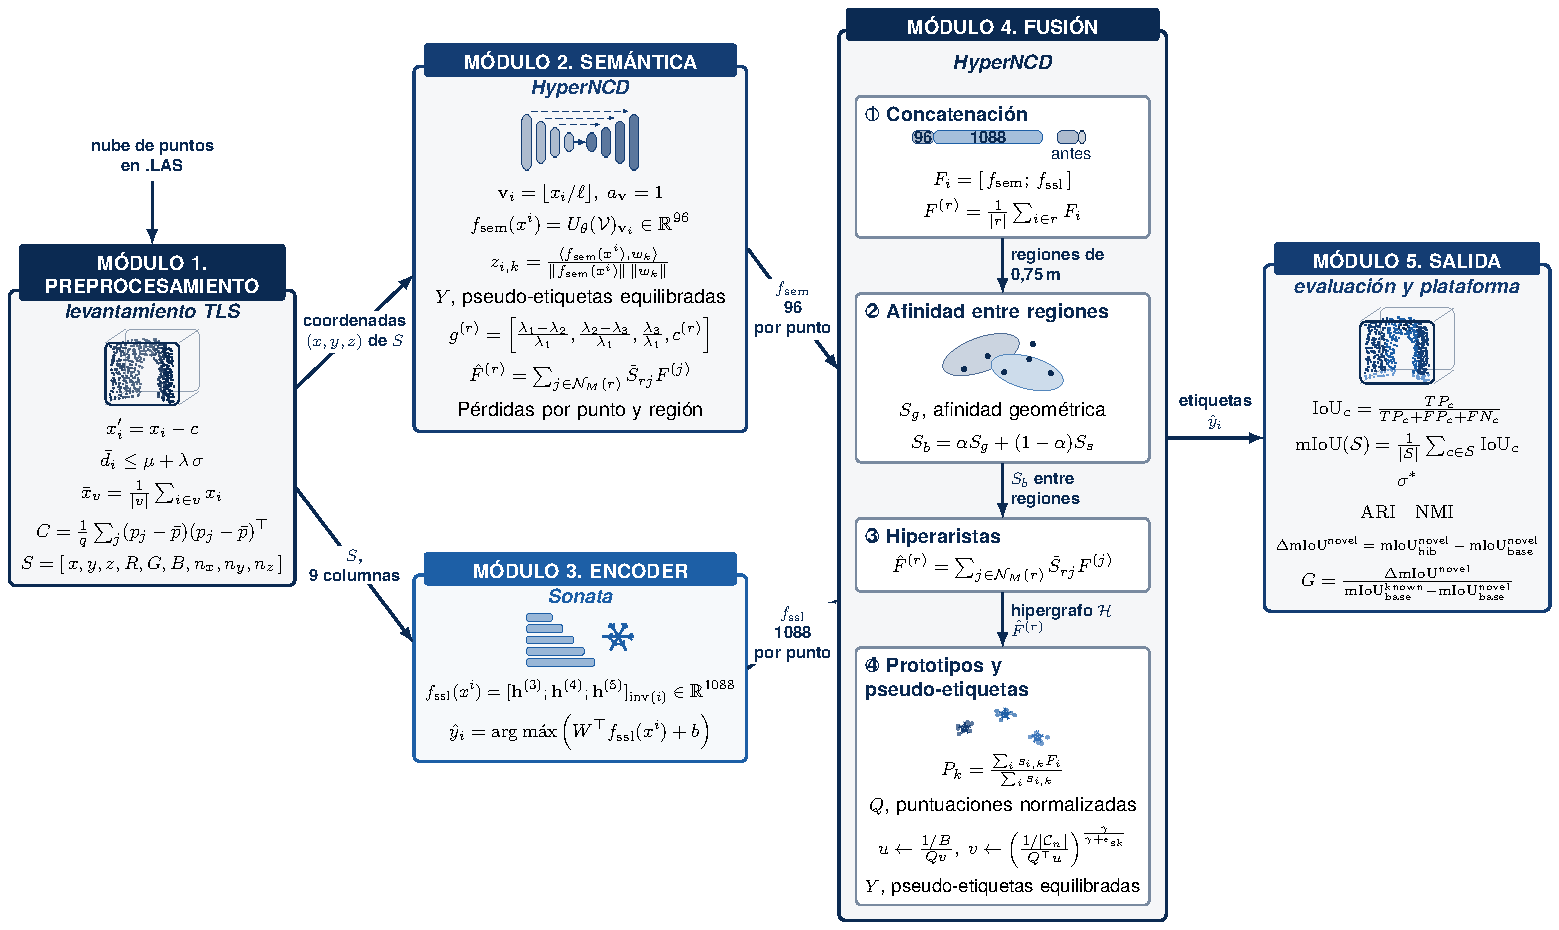
\includegraphics[width=278mm,height=208mm,keepaspectratio]{fig/diagrama_poster.pdf}};

% --- Bloque 4: La capilla por metodo (Etiquetas y leyenda en vectorial) -----
\caja{226}{314}{290}{248}{white}
\seccion{226}{314}{290}{4}{La capilla por método}

% Rotulos laterales en vectorial (Planta y Vista lateral)
\node[rotate=90,font=\tit\fs{13.5}{16},text=navy] at (236,396) {Planta $(x, y)$};
\node[rotate=90,font=\tit\fs{13.5}{16},text=navy] at (236,488) {Vista lateral $(x, z)$};

% Los 5 paneles en planta y vista lateral con encabezados vectoriales nitidos
\foreach \i/\f/\n/\m in {0/real/Etiqueta real/5 clases,1/m2/M2/{\mioun\ 49,0\,\%},2/m3/M3/{\mioun\ 52,5\,\%},3/m4base/M4 base/{\mioun\ 52,9\,\%},4/m4/M4 híbrido/{\mioun\ 50,6\,\%}}{
  \pgfmathsetmacro{\xc}{268+\i*53}
  \node[font=\tit\fs{13.5}{15.5},text=navy] at (\xc,343) {\n};
  \node[font=\fs{11.5}{13.5},text=suave] at (\xc,350) {(\m)};
  \draw[borde,line width=.35mm,rounded corners=1mm] (\xc-23,355) rectangle (\xc+23,438);
  \node[anchor=center,inner sep=0] at (\xc,396.5) {\includegraphics[height=79mm,width=43mm,keepaspectratio]{fig/planta_\f.png}};
  \draw[borde,line width=.35mm,rounded corners=1mm] (\xc-23,444) rectangle (\xc+23,530);
  \node[anchor=center,inner sep=0] at (\xc,487) {\includegraphics[height=82mm,width=43mm,keepaspectratio]{fig/lateral_\f.png}};
}

% Leyenda grande y nitida de las clases en la base del Bloque 4
\fill[tesela,draw=borde,line width=.3mm,rounded corners=1.5mm] (236,536) rectangle (506,555);
\foreach \x/\c/\t in {248/D62728/Arco,290/1F77B4/Columna,342/FF7F0E/Cúpula,392/2CA02C/Pared,438/9467BD/Techo,482/4D4D4D/Sin clase}{
  \definecolor{cl}{HTML}{\c}\fill[cl] (\x,545.5) circle[radius=2.8mm];
  \node[anchor=west,inner sep=0,font=\tit\fs{13}{15},text=tinta] at (\x+4.5,545.5) {\t};}

% ============================================================================
% COLUMNA 3 (DERECHA: x = 522, w = 303 mm)
% 5. Comparacion de los cuatro modelos | 6. Descubrimiento por clase | 7. Umbral de 70%
% ============================================================================

% --- Bloque 5: Comparacion de los cuatro modelos ----------------------------
\caja{522}{70}{303}{156}{white}
\seccion{522}{70}{303}{5}{Comparación de los cuatro modelos}

\node[anchor=north west,inner sep=0] at (528,93)
  {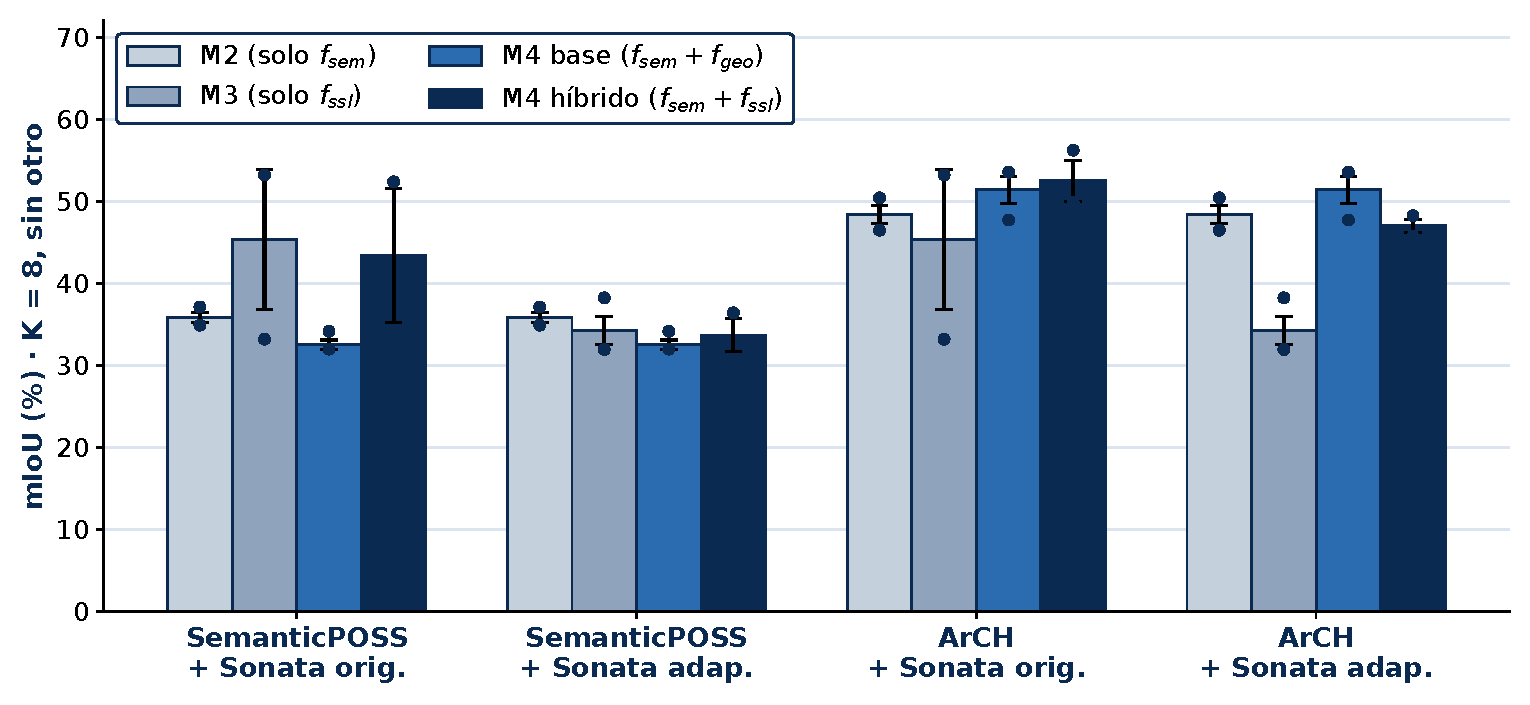
\includegraphics[width=178mm]{fig/poster_m4_semillas.pdf}};

\fill[tesela,draw=borde,line width=.3mm,rounded corners=1.6mm] (710,95) rectangle (816,175);
\node[anchor=north west,inner sep=0,font=\tit\fs{12.5}{15},text=navy] at (715,99)
  {Capilla, 10 semillas ($K=8$)};
\node[anchor=north west,inner sep=0,font=\fs{11.5}{14.2},text=tinta] at (714,107) {%
  \setlength{\tabcolsep}{3.5pt}
  \begin{tabular}{@{}lrr@{}}
  \toprule
  \textbf{Modelo} & \textbf{\miou\ (\%)} & \textbf{Cambio} \\
  \midrule
  M2 SemPOSS & $35{,}9\pm0{,}6$ & --- \\
  M2 ArCH & $48{,}4\pm1{,}1$ & $+12{,}5$ \\
  M3 Sonata orig. & $45{,}4\pm8{,}5$ & --- \\
  M3 Sonata adap. & $34{,}3\pm1{,}7$ & $-11{,}1$ \\
  M4 base & $51{,}4\pm1{,}7$ & --- \\
  \textbf{M4 híbrido} & $\mathbf{52{,}5\pm2{,}5}$ & $+1{,}1$ \\
  \bottomrule
  \end{tabular}};

\cuerposm{532}{180}{282}{%
  \punto{Con M2 de ArCH, la fusión sube de 45{,}4\,\% (M3) y 48{,}4\,\% (M2) a \textbf{52{,}5\,\% (M4)}, bajando la desviación de M3 de $\pm 8{,}5$ a $\pm 2{,}5$. Adaptar Sonata con lote de una escena redujo su rango efectivo de 97{,}7 a 64{,}3.}
  \punto{En 39 variantes de fusión, ninguna supera al pegado normalizado con M2 de ArCH ($-0{,}2$ a $+1{,}1$ puntos), aunque con M2 colapsado rescatan hasta $+18{,}2$ puntos.}
}

% --- Bloque 6: Descubrimiento por clase y cabezas de M2 ---------------------
\caja{522}{232}{303}{168}{white}
\seccion{522}{232}{303}{6}{Descubrimiento por clase y cabezas de M2}

\node[anchor=north west,inner sep=0] at (528,255)
  {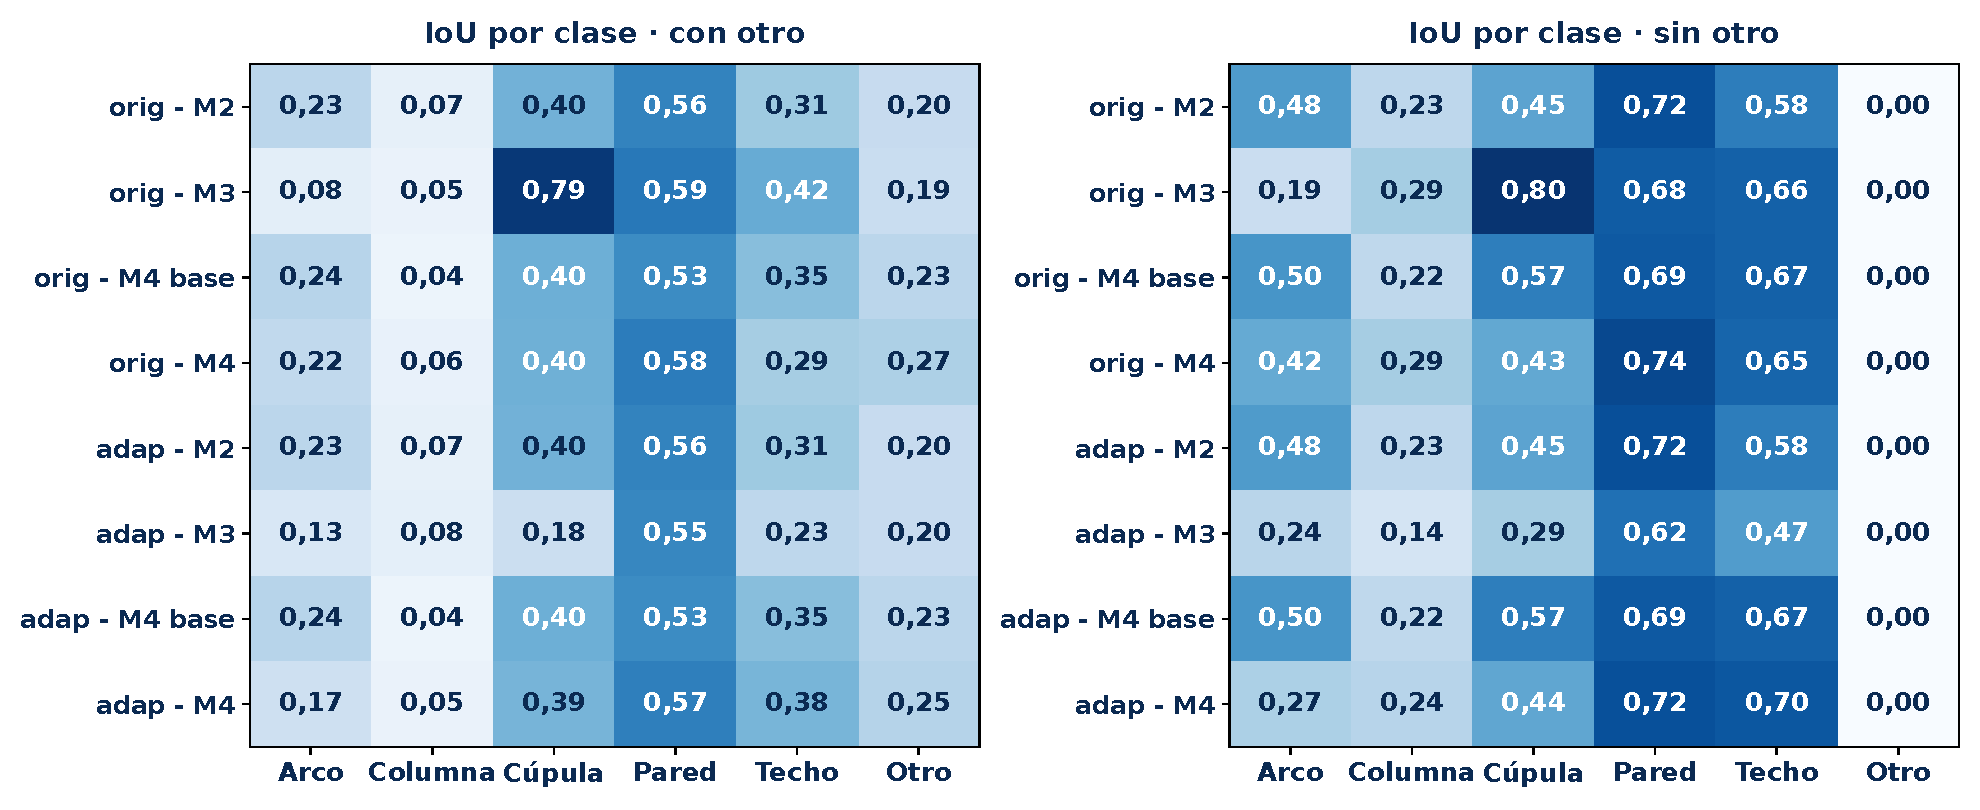
\includegraphics[width=158mm]{fig/poster_m4_iou_por_clase.pdf}};

\node[anchor=north west,inner sep=0] at (690,255)
  {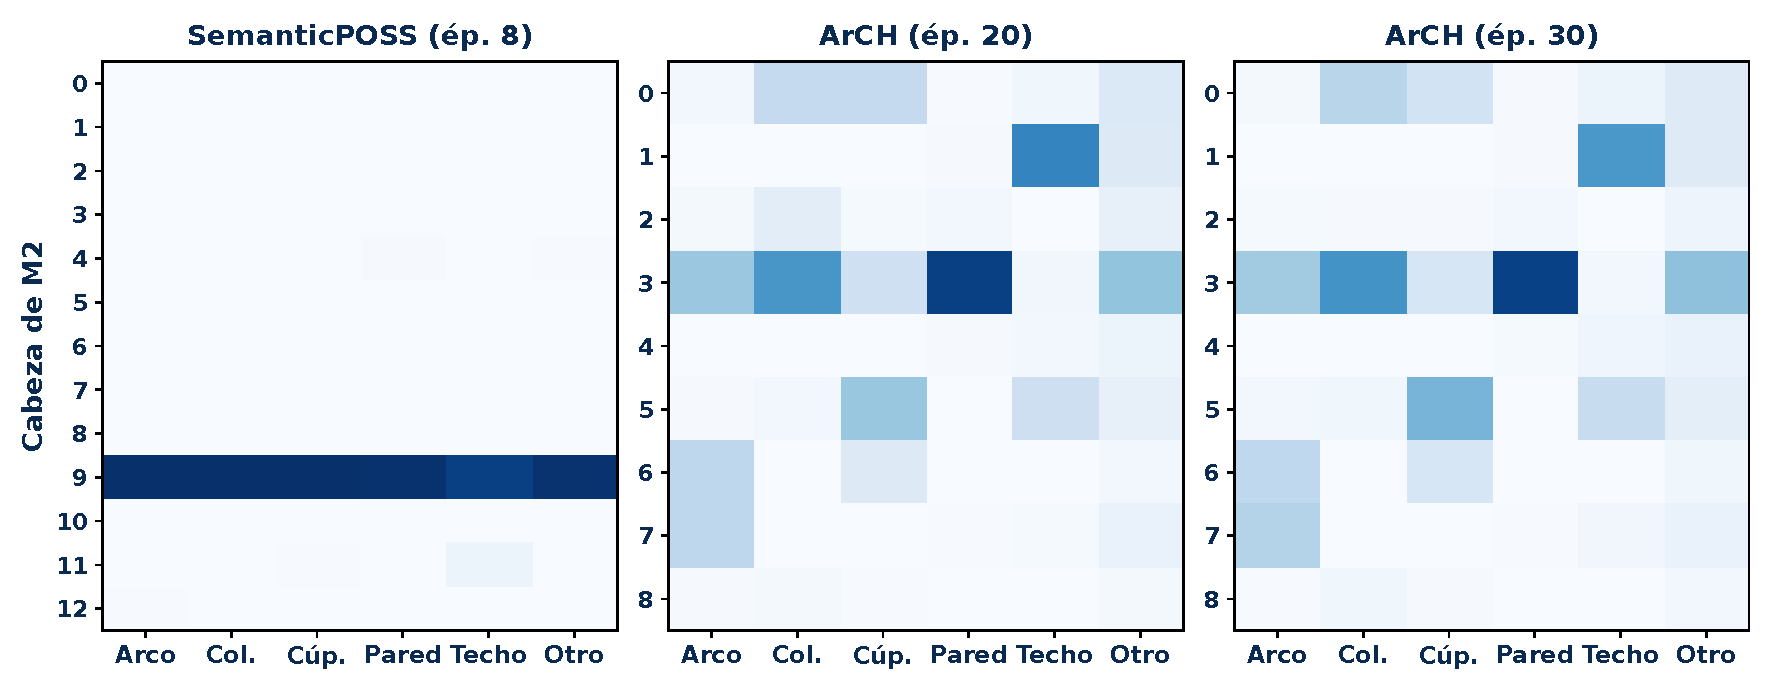
\includegraphics[width=126mm]{fig/poster_m2_cabeza_x_clase.pdf}};

\fill[tesela,draw=borde,line width=.3mm,rounded corners=1.5mm] (690,309) rectangle (816,352);
\node[anchor=north west,inner sep=0,font=\tit\fs{12}{14},text=navy] at (695,312)
  {\iou\ por clase (\%) y sonda lineal};
\node[anchor=north west,inner sep=0,font=\fs{11.2}{13.6},text=tinta] at (695,319) {%
  \setlength{\tabcolsep}{3.8pt}
  \begin{tabular}{@{}lrrrrr@{}}
  \toprule
  \textbf{Método} & \textbf{Arco} & \textbf{Col.} & \textbf{Cúp.} & \textbf{Pared} & \textbf{Techo} \\
  \midrule
  M3 orig. & 18,7 & 28,9 & \textbf{80,5} & 68,2 & 66,4 \\
  M2 ArCH & 48,0 & 22,6 & 44,8 & 72,1 & 57,5 \\
  M4 orig. & 42,3 & 28,6 & 43,0 & \textbf{74,2} & 65,1 \\
  \textbf{Sonda} & \textbf{70,8} & \textbf{66,4} & \textbf{89,5} & \textbf{91,2} & \textbf{89,0} \\
  \bottomrule
  \end{tabular}};

\cuerposm{532}{357}{282}{%
  \punto{\textbf{M3} destaca en \textbf{cúpula (80{,}5\,\% de~\ioun, precisión 97{,}4\,\%)}, pero falla en \textbf{arco (18{,}7\,\%)}. \textbf{M2 con ArCH} recupera el \textbf{arco (48{,}0\,\%)} y en \textbf{M4} logra el máximo en \textbf{pared (74{,}2\,\%)}, pero baja el recall de la cúpula de 82{,}3\,\% a 46{,}7\,\%. La \textbf{columna (22--29\,\%)} absorbe falsos positivos de piezas vecinas.}
}

% --- Bloque 7: Umbral de 70% y dificultad por clase -------------------------
\caja{522}{406}{303}{156}{white}
\seccion{522}{406}{303}{7}{Umbral de 70\,\% y dificultad por clase}

\node[anchor=north west,inner sep=0] at (528,428)
  {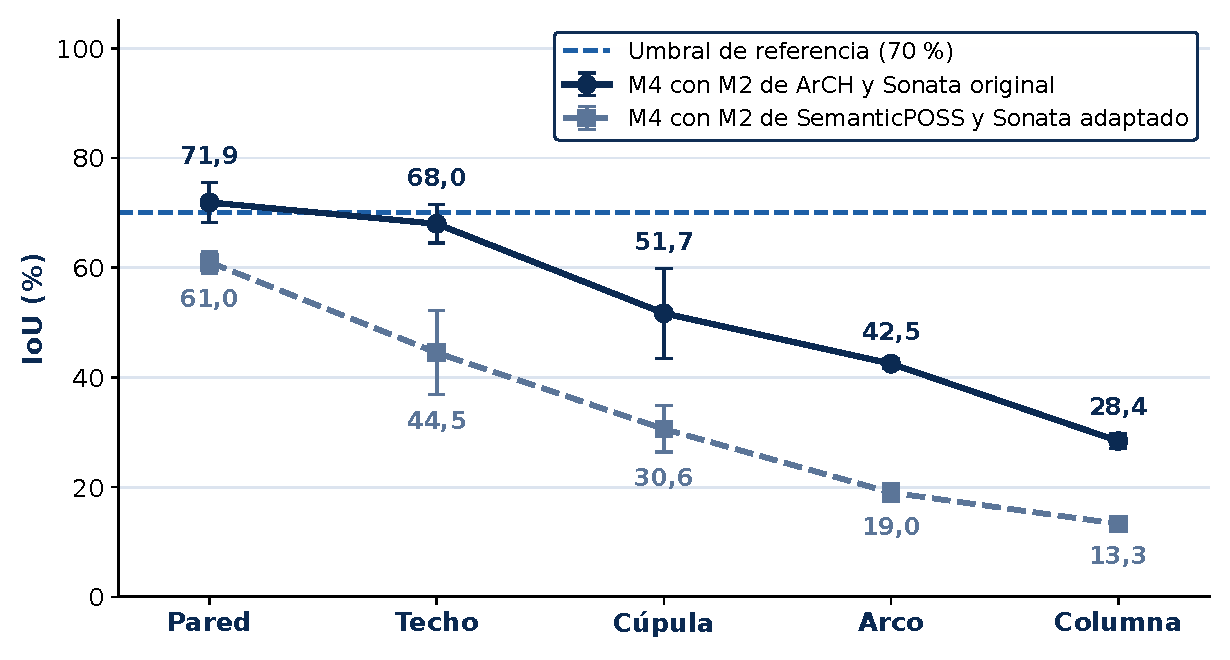
\includegraphics[width=156mm]{fig/poster_umbral.pdf}};

\node[anchor=north west,inner sep=0,text width=126mm,align=left,font=\fs{12.4}{16.0},text=tinta] at (688,430)
  {\rg Se eligió un umbral de 70\,\% de~\ioun\ porque las clases principales en ArCH (72{,}1\,\% a 88{,}7\,\%), la sonda lineal (70{,}8\,\% a 91{,}2\,\%) y Sonata en interiores (72{,}6\,\% a 77{,}6\,\%) superan ese nivel. El orden de dificultad sigue al tamaño de cada clase ($\rho=+0{,}90$) y es inverso a su linealidad ($\rho=-0{,}90$).};

\fill[tesela,draw=borde,line width=.3mm,rounded corners=1.4mm] (688,496) rectangle (816,554);
\node[anchor=north west,inner sep=0,font=\fs{11.4}{14.2},text=tinta] at (693,500) {%
  \setlength{\tabcolsep}{4.2pt}
  \begin{tabular}{@{}lrrr@{}}
  \toprule
  \textbf{Clase} & \textbf{\iou\ M4 (\%)} & \textbf{Escena (\%)} & \textbf{Linealidad} \\
  \midrule
  Pared & $71{,}9\pm3{,}6$ & 15,3 & 0,194 \\
  Techo & $68{,}0\pm3{,}5$ & 6,6 & 0,198 \\
  Cúpula & $51{,}7\pm8{,}2$ & 9,7 & 0,272 \\
  Arco & $42{,}5\pm0{,}9$ & 4,2 & 0,380 \\
  Columna & $28{,}4\pm1{,}3$ & 2,9 & 0,351 \\
  \bottomrule
  \end{tabular}};

% ============================================================================
% BANDA DE PIE DE PAGINA (y = 568 a 594 mm)
% ============================================================================
\fill[navy] (0,568) rectangle (841,594);
\fill[azul] (0,568) rectangle (841,570);
\node[anchor=west,inner sep=0,text=white,font=\fs{13.5}{16.5}] at (18,581.5)
  {Basado en HyperNCD (Zhang et al., CVPR 2026), Sonata (Wu et al., CVPR 2025) y el conjunto ArCH (Matrone et al., ISPRS 2020)};
\end{tikzpicture}
\end{lrbox}
\AddToShipoutPictureBG*{\AtPageUpperLeft{\vbox to 0pt{\hbox{\scalebox{1.413793}{\usebox{\cartel}}}\vss}}}
\null
\end{document}
